\documentclass[xcolor=svgnames,handout]{beamer}

\usepackage[utf8]    {inputenc}
\usepackage[T1]      {fontenc}
\usepackage[english] {babel}

\usepackage{amsmath,amsfonts,graphicx}
\usepackage{beamerleanprogress}


\title
  [Short Title\hspace{2em}]
  {Machine Learning techniques for predicting molecular properties}

\author
  [Viviana Petrescu]

\date
  {April 01, 2011}

\institute
  {Justice League of America}


\begin{document}

\maketitle

\section
  {Introduction}
%%%%%%%%%%%%%%%%%%%%%%%%%%%%%%%%%%%%%%%%%%%%%%%%%%%%%%
\begin{frame}{Introduction}
\tableofcontents
\end{frame}

\begin{frame}
  {Introduction}

  Things in a Bulleted List\pause

  \begin{itemize}
  \item Bullets that\pause
  \item Come up\pause
  \item One by one
  \end{itemize}
\end{frame}



\section
  {Main Body}

\begin{frame}
  {Equations}

  Equations are easy
  \begin{itemize}
  \item Just copy/paste equations\pause
  \item From the paper!
    \begin{equation*}
      \textbf{p}^* = \underset{\textbf{p}}{\arg\!\min}~\sum_{\textbf{x}}\left[ I(\textbf{W}(\textbf{x};\textbf{p})) - T(\textbf{x}) \right]^2
    \end{equation*}
  \end{itemize}
\end{frame}


\begin{frame}
  {Pictures}

  \begin{figure}[t]
    \centering
    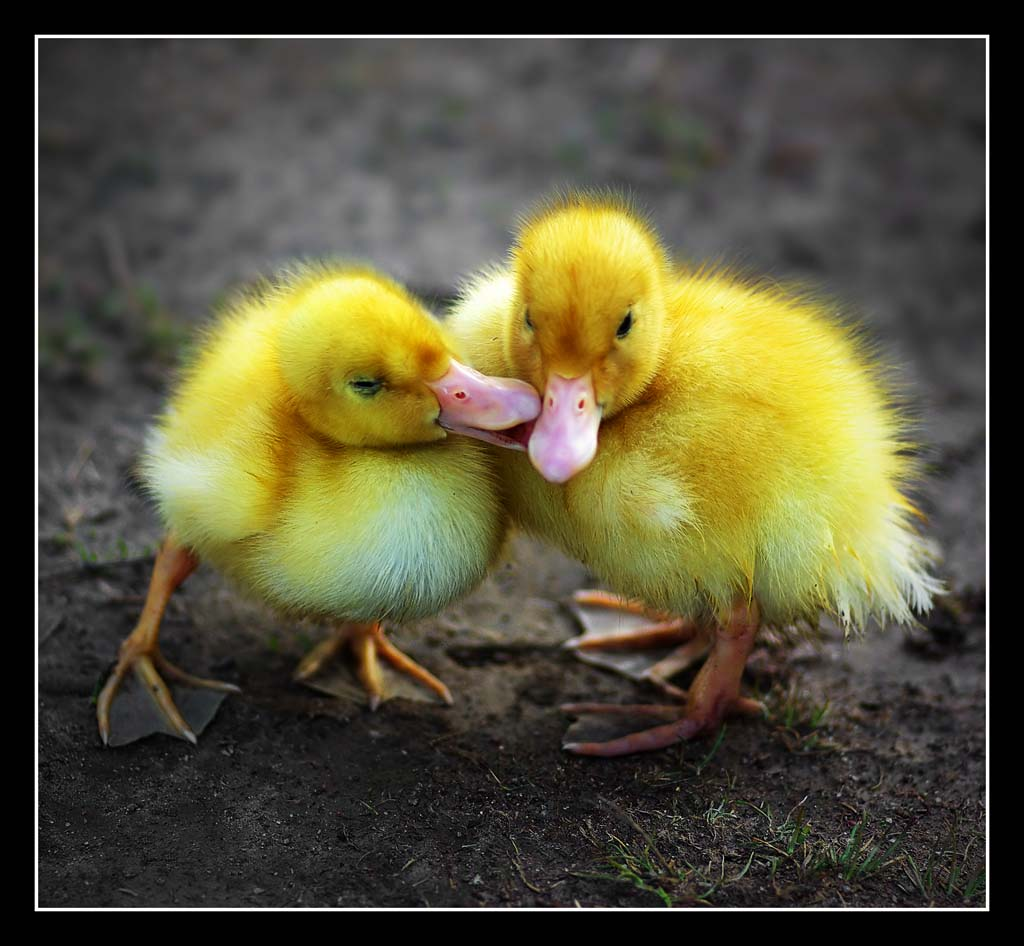
\includegraphics[height=\dimexpr11\textheight/16\relax]{ducks}
    \caption{Kissing ducks}
  \end{figure}
\end{frame}


\begin{frame}
  {A Movie}

  \begin{block}{Some block}
    \begin{itemize}
    \item Movies only seem to work in Adobe Reader
    \item Movie file is not embedded, it must be on the computer
    \end{itemize}
  \end{block}

  \begin{exampleblock}{Some more block}
    Movies only seem to work in Adobe Reader\par
    Movie file is not embedded, it must be on the computer
  \end{exampleblock}

  \begin{alertblock}{}
    Some text in here.
    \begin{itemize}
    \item Movies only seem to work in Adobe Reader
    \item Movie file is not embedded, it must be on the computer
    \end{itemize}
  \end{alertblock}
\end{frame}



\section
  {Conclusion}

\begin{frame}
  {Credits}

  \begin{itemize}
  \item Brought to you by Cédric Mauclair
  \item Please let me know about improvements!
  \item inspiration: \url{http://www.shawnlankton.com}... (in code)
  \end{itemize}
\end{frame}


\begin{frame}
  {Questions}

  \nocite{lorem,ipsum}
  \bibliographystyle{plain}
  \bibliography{demo}

\end{frame}

\end{document}

